\documentclass[a4paper,12pt]{report}

\usepackage[italian]{babel}
\usepackage[utf8]{inputenc}
\usepackage[T1]{fontenc}
\usepackage{graphicx}
\usepackage{float}
\usepackage{pdfpages}
\restylefloat{table}
%\usepackage[style=numeric-comp]{biblatex}

\title{InfoTreno}
\author{Chelli M. \thanks{michael.chelli@studio.unibo.it - 915585}, Tampieri E.\thanks{eugenio.tampieri@studio.unibo.it - 915602} - Gruppo 2098}

\begin{document}
	\maketitle
	\tableofcontents
	\chapter{Analisi dei requisiti}
	\section{Intervista}
	\par RFS (Rete Ferroviaria dello Stato) richiede la realizzazione di un sistema informativo in grado di monitorare la marcia e la programmazione dei treni e la gestione dei turni del personale di bordo. Viene richiesta la possibilità di operare tramite interfaccia web, in modo da essere indipendenti dalle piattaforme utilizzate.
	\par Un treno è uno specifico viaggio su una relazione, ovvero l'attraversamento sequenziale di una serie di punti di passaggio (scambi, stazioni, o semplici) in orari predeterminati.
	\par Oltre alla memorizzazione degli orari di attraversamento teorici, viene richiesta la memorizzazione della data e ora di partenza e di arrivo da un punto di passaggio, così da poter calcolare il ritardo del treno.
	\par Un treno è poi composto da una locomotiva (della quale ci interessa conoscere la velocità e la tensione di esercizio) e una serie di carrozze (delle quali ci interessa memorizzare la classe e il numero di posti), che formano un convoglio.
	\par Su un treno prendono servizio un macchinista, un capotreno e, in certi casi, dei controllori.

	\section{Rilevamento delle ambiguità e correzioni proposte}
	\par RFS (Rete Ferroviaria dello Stato) richiede la realizzazione di un sistema informativo in grado di monitorare la marcia e la programmazione dei treni e la gestione dei turni del personale di bordo. Viene richiesta la possibilità di operare\textsuperscript{1} tramite interfaccia web, in modo da essere indipendenti dalle piattaforme utilizzate.
	\par Un treno è uno specifico viaggio su una linea ferroviaria, ovvero l'attraversamento sequenziale di una serie di punti di passaggio\textsuperscript{2} (scambi, stazioni, o semplici\textsuperscript{3}) in orari predeterminati.
	\par Oltre alla memorizzazione degli orari di attraversamento teorico, viene richiesta la memorizzazione della data e ora di partenza e di arrivo da un punto di passaggio, così da poter calcolare il ritardo del treno.
	\par Un treno è poi composto da una locomotiva (della quale ci interessa conoscere la velocità e la tensione di esercizio) e una serie di carrozze (delle quali ci interessa memorizzare la classe\textsuperscript{4} e il numero di posti), che formano un convoglio.
	\par Su un treno prendono servizio un macchinista, un capotreno e, in certi casi, dei controllori.

	\begin{tabular}{|p{1cm}|p{3cm}|p{4cm}|p{4cm}|}
		\hline
		\textbf{N} & \textbf{Espressione} & \textbf{Sostituzione} & \textbf{Motivazione} \\ \hline
		1 & Operare & Interagire con il sistema & Esplicitato il concetto  \\ \hline
		2 & Punti di passaggio & rappresentati nel mondo fisico da eurobalise & specificato il significato \\ \hline
		3 & Semplici & in tutti gli altri casi & specificato il significato \\ \hline
		4 & classe & classe (prima o seconda) & specificato il significato \\ \hline
	\end{tabular}

	\subsection{Dopo la correzione delle ambiguità}
	\par RFS (Rete Ferroviaria dello Stato) richiede la realizzazione di un sistema informativo in grado di monitorare la marcia e la programmazione dei treni e la gestione dei turni del personale di bordo. Viene richiesta la possibilità di interagire con il sistema tramite interfaccia web, in modo da essere indipendenti dalle piattaforme utilizzate.
	\par Un treno è uno specifico viaggio su una linea ferroviaria, ovvero l'attraversamento sequenziale di una serie di punti di passaggio, rappresentati nel mondo fisico da eurobalise (scambi, stazioni, o semplici, in tutti gli altri casi) in orari predeterminati.
	\par Oltre alla memorizzazione degli orari di attraversamento teorico, viene richiesta la memorizzazione della data e ora di partenza e di arrivo da un punto di passaggio, così da poter calcolare il ritardo del treno.
	\par Un treno è poi composto da una locomotiva (della quale ci interessa conoscere la velocità e la tensione di esercizio) e una serie di carrozze (delle quali ci interessa memorizzare la classe, prima o seconda, e il numero di posti), che formano un convoglio.
	\par Su un treno prendono servizio un macchinista, un capotreno e, in certi casi, dei controllori.

	\section{Definizione delle specifiche in linguaggio naturale ed estrazione dei concetti principali}
	\par Si individuano le parole chiave che permetteranno di costruire un primo schema scheletro del progetto. In seguito sarà poi raffinato per ottenere lo schema definitivo. I termini essenziali sono evidenziati in grassetto e in corsivo.
	\par RFS (Rete Ferroviaria dello Stato) richiede la realizzazione di un sistema informativo in grado di monitorare la marcia e la programmazione dei treni e la gestione dei turni del personale di bordo. Viene richiesta la possibilità di interagire con il sistema tramite interfaccia web, in modo da essere indipendenti dalle piattaforme utilizzate.
	\par Un \textbf{\textit{treno}} è uno specifico viaggio su una linea ferroviaria, ovvero l'attraversamento sequenziale di una serie di \textbf{\textit{punti di passaggio}}, rappresentati nel mondo fisico da eurobalise (scambi, stazioni, o semplici, in tutti gli altri casi) in orari predeterminati.
	\par Oltre alla memorizzazione degli \textbf{\textit{orari di attraversamento}} teorico, viene richiesta la memorizzazione della \textbf{\textit{data e ora di partenza e di arrivo}} da un punto di passaggio, così da poter calcolare il ritardo del treno.
	\par Un treno è poi composto da una \textbf{\textit{locomotiva}} (della quale ci interessa conoscere la velocità e la tensione di esercizio) e una serie di \textbf{\textit{carrozze}} (delle quali ci interessa memorizzare la classe (prima o seconda) e il numero di posti), che formano un \textbf{\textit{convoglio}}.
	\par Su un treno prendono servizio un macchinista, un capotreno e, in certi casi, dei controllori.
% ____                           _   _               _
%|___ \  ___ ___  _ __   ___ ___| |_| |_ _   _  __ _| | ___
%  __)  / __/ _ \| '_ \ / __/ _ | __| __| | | |/ _` | |/ _ \
% / __/| (_| (_) | | | | (_|  __| |_| |_| |_| | (_| | |  __/
%|_____ \___\___/|_| |_|\___\___|\__|\__|\__,_|\__,_|_|\___|
	\chapter{Progettazione concettuale}
	\par In questa situazione il dominio è specifico ed è spesso possibile trovare delle entità generiche che si concretizzano poi in entità più specifiche. Per questo motivo è utile utilizzare un approccio top-down per modellare al meglio l'architettura.
	\section{Schema scheletro}
	\begin{figure}[h]
		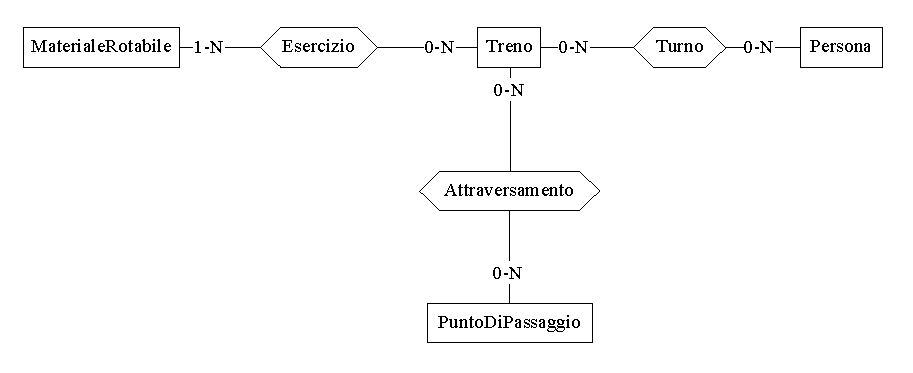
\includegraphics[width=\linewidth]{res/schema/skel}
		\caption{Schema scheletro}
	\end{figure}
	\section{Raffinamenti proposti}
	\par Lo schema concettuale sarà sviluppato perfezionando tutte le entità nello schema scheletro. Per ogni entità si propone di seguito una vista esplosa, l'unione delle quali condurrà allo schema finale.
	\subsection{Entità \textit{MaterialeRotabile}}
	\begin{figure}[h]
		\begin{center}
			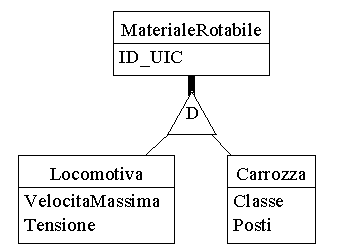
\includegraphics{res/schema/loco}
		\end{center}
		\caption{Gerarchia di MaterialeRotabile}
		\label{fig:loco}
	\end{figure}
	\par Il materiale rotabile viene suddiviso in locomotive e carrozze (fig. \ref{fig:loco}), lasciando eventualmente spazio ad altri tipi di materiale rotabile quali i carri merci.
	\par Al contempo, si vuole differenziare la relazione fra una carrozza e una locomotiva, facendo in modo che ci possa essere solo una locomotiva per ogni convoglio (fig. \ref{fig:esercizio}). Per ottenere ciò viene aggiunta una entità chiamata \textit{Convoglio}, alla quale vengono messi in relazione una \textit{Locomotiva} e zero o più \textit{Carrozze}. Alla fine del raffinamento, viene sostituita la relazione fra \textit{Treno} e \textit{MaterialeRotabile} con una relazione fra \textit{Treno} e \textit{Convoglio} che a sua volta è collegato alle entità gerarchicamente figlie di \textit{Materiale rotabile}.
	\begin{figure}[h!]
		\begin{center}
			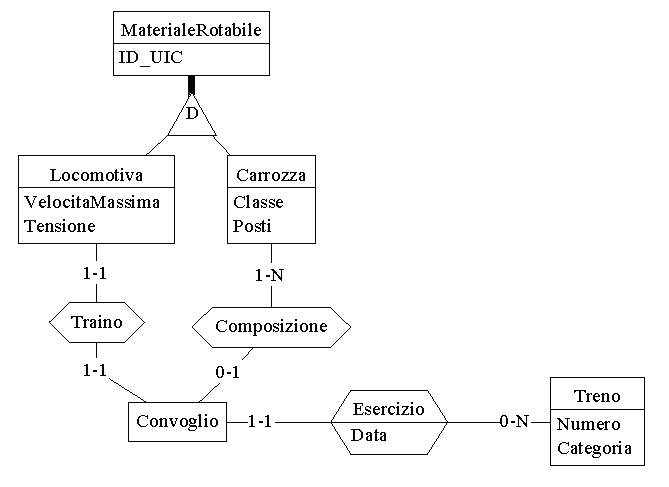
\includegraphics[scale=0.75]{res/schema/esercizio}
		\end{center}
		\caption{La relazione esercizio con le relative entità}
		\label{fig:esercizio}
	\end{figure}
	\subsection{Entità \textit{PuntoDiPassaggio}}
	\begin{figure}[h!]
		\begin{center}
			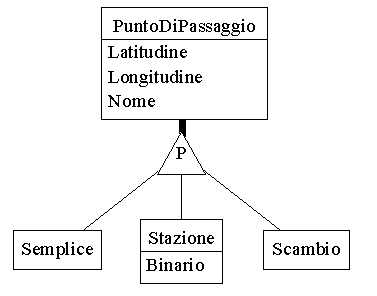
\includegraphics{res/schema/pdp}
		\end{center}
		\caption{Gerarchia sui punti di passaggio}
		\label{fig:pdp}
	\end{figure}
	\begin{figure}[h!]
		\begin{center}
			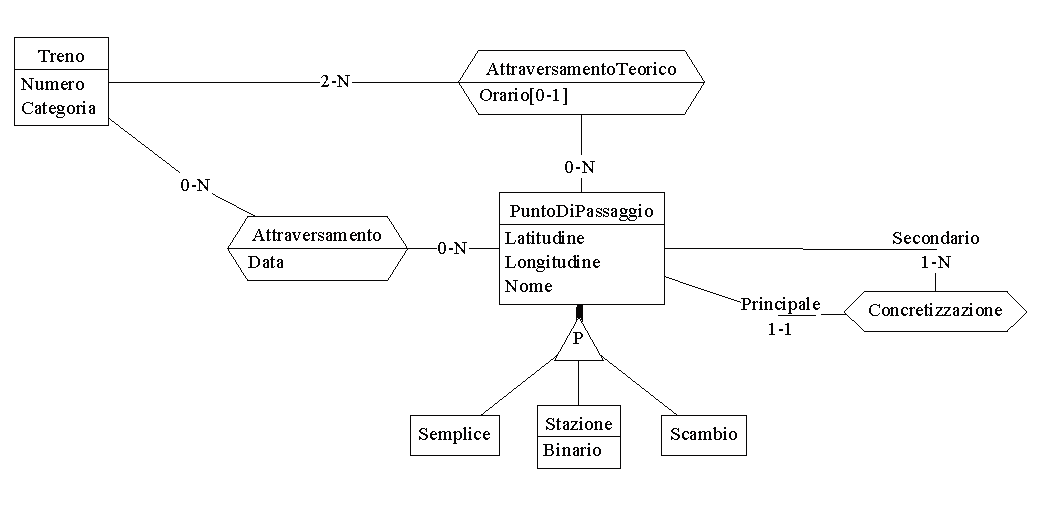
\includegraphics[width=\linewidth]{res/schema/attraversamento}
		\end{center}
		\caption{La relazione \textit{Attraversamento} con le relative entità}
		\label{fig:attraversamento}
	\end{figure}
	\par Per quanto riguarda l'entità \textit{PuntoDiPassaggio}, viene innanzitutto introdotta una gerarchia (fig. \ref{fig:pdp}), principalmente per modellare la fermata su uno specifico binario in una stazione.
	\par Questa gerarchia ci consente anche di modellare gli scambi che, sebbene non abbiano particolare rilevanza in questo progetto, da la possibilità di controllare eventuali situazioni di pericolo in prossimità degli scambi e ottenere la lista di operazioni da effettuare su uno scambio per consentire la corretta configurazione della linea ferroviaria.
	\par Inoltre, vengono introdotte due nuove relazioni (\textit{Concretizzazione} ed \textit{AttraversamentoTeorico}, fig. \ref{fig:attraversamento}).
	\par La seconda ci permette di definire delle tabelle di marcia, ovvero contenenti solo gli orari di attraversamento di uno specifico punto di passaggio, mentre la prima fa sì che si possano definire dei gruppi di punti di passaggio, in modo da poter definire l'\textit{AttraversamentoTeorico} sul \textit{PuntoDiPassaggio} principale, mentre l'\textit{Attraversamento} avviene sui punti di passaggio secondari.
	\par Questa suddivisione torna particolarmente utile quando un treno, che secondo l'orario dovrebbe arrivare a un binario, arriva su un binario diverso.
	\subsection{Entità \textit{Persona}}
	\begin{figure}[h!]
		\begin{center}
			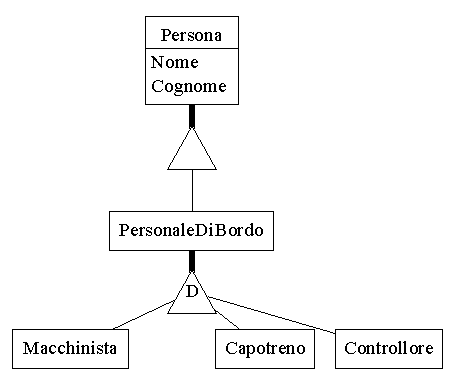
\includegraphics{res/schema/persona}
		\end{center}
		\caption{Gerarchia su Persona}
		\label{fig:persona}
	\end{figure}
	\begin{figure}[h!]
		\begin{center}
			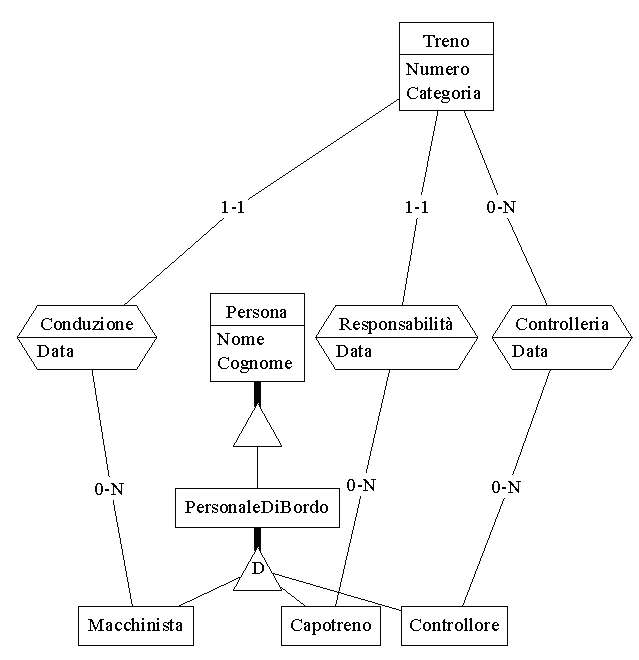
\includegraphics[scale=.75]{res/schema/turno}
		\end{center}
		\caption{Le entità e le relazioni necessarie alla modellazione di un turno}
		\label{fig:turno}
	\end{figure}
	\par Nel dominio applicativo, l'entità \textit{Persona} presente nello schema scheletro è sicuramente molto generica. Questo ci consente di introdurre una gerarchia (fig. \ref{fig:persona}) parziale che ci permetterebbe in futuro di modellare anche i biglietti comprati dai clienti.
	\par In \textit{PersonaleDiBordo} viene a sua volta inserita una gerarchia, per poter distinguere fra i ruoli che una persona svolge.
	\par Questo ci consente (fig. \ref{fig:turno}) di poter specificare il personale minimo e massimo su ogni treno.
	\section{Schema concettuale finale}
	\begin{figure}[h!]
		\begin{center}
			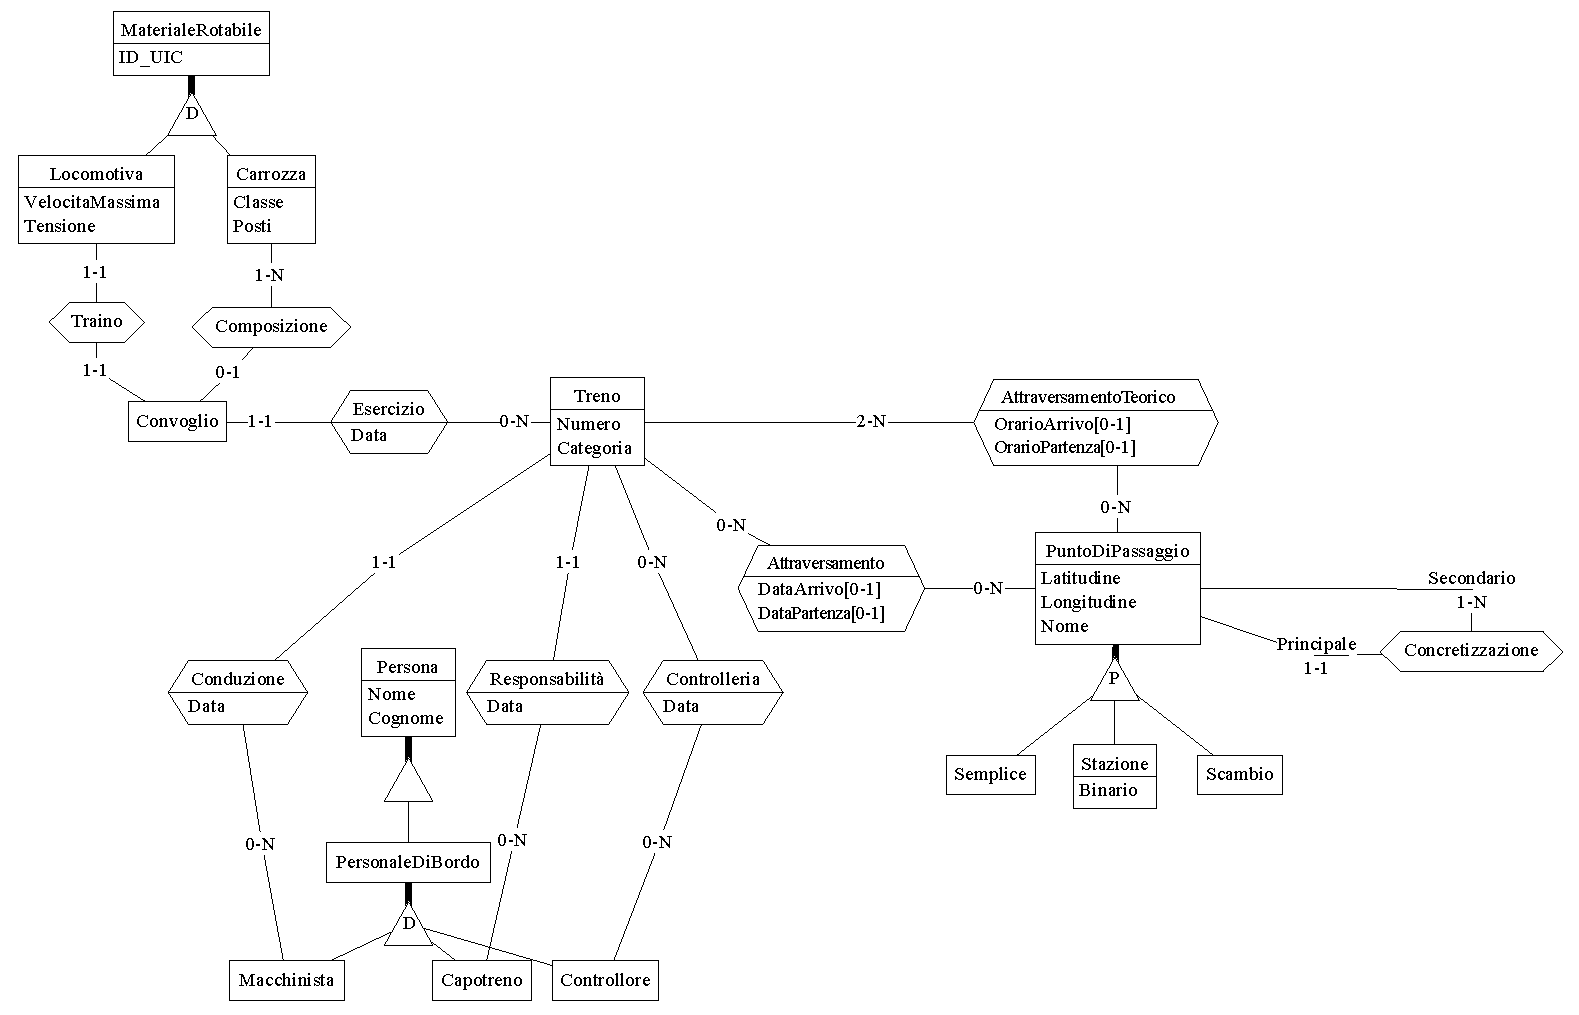
\includegraphics[angle=270,width=.95\linewidth]{res/schema/full}
		\end{center}
		\caption{Schema concettuale finale}
	\end{figure}
	\chapter{Progettazione logica}
	\section{Stima del volume dei dati}
	\par Si ripoerao le stime dei volumi dei dati dopo un anno di operatività.
	\begin{table}[H]
	\centering
	\begin{tabular}{|l|l|l|}
		\hline \textbf{Nome} & \textbf{Tipo} & \textbf{Volume} \\
		\hline Treno & E & 30000 \\
		\hline PuntoDiPassaggio & E & 10000 \\
		\hline Stazione & E & 1000 \\
		\hline Semplice & E & 6000 \\
		\hline Scambio & E & 3000 \\
		\hline Concretizzazione & R & 50000 \\
		\hline AttraversamentoTeorico & E & 9000000 \\
		\hline Attraversamento & E & 3285000000 \\
		\hline Persona & E & 50000 \\
		\hline PersonaleDiBordo & E & 50000 \\
		\hline Macchinista & E & 12500 \\
		\hline Conduzione & R & 10950000 \\
		\hline Capotreno & E & 12500 \\
		\hline Responsabilit\`a & R & 10950000 \\
		\hline Controllore & E & 25000 \\
		\hline Controlleria & R & 10950000 \\
		\hline MaterialeRotabile & E & 60000 \\
		\hline Locomotiva & E & 10000 \\
		\hline Traino & R & 20000 \\
		\hline Carrozza & E & 50000 \\
		\hline Composizione & R & 50000 \\
		\hline Convoglio & E & 20000 \\
		\hline Esercizio & R & 10950000 \\
		\hline
	\end{tabular}
	\end{table}
	\section{Descrizione delle operazioni principali e stima della loro frequenza}
	Di seguito si riportano le operazioni effettuate e la stima della loro frequenza dopo un anno di operatività.
	\begin{table}[H]
	\centering
	\begin{tabular}{|l|l|l|}
		\hline \textbf{N} & \textbf{Descrizione} & \textbf{Frequenza} \\
		\hline 1 & Treno: inserimento & 1/settimana \\
		\hline 2 & PuntoDiPassaggio: inserimento & 1/mese \\
		\hline 3 & AttraversamentoTeorico: inserimento & 1/giorno \\
		\hline 4 & Attraversamento: inserimento & 9000000/giorno \\
		\hline 5 & Persona: inserimento & 3/mese \\
		\hline 6 & Esercizio: inserimento & 20000/giorno \\
		\hline 7 & Convoglio: inserimento & 1/giorno \\
		\hline 8 & Locomotiva: inserimento & 1/mese \\
		\hline 9 & Carrozza: inserimento & 5/mese \\
		\hline 10 & Ricerca stazione: interrogazione & 2000000/giorno \\
		\hline 11 & Lista treni: interrogazione & 2000000/giorno \\
		\hline 12 & Ritardo treno: interrogazione & 2000000/giorno \\
		\hline 13 & Stazione treno: interrogazione & 2000000/giorno \\
		\hline 14 & Attraversamenti Teorici treno: interrogazione & 2000000/giorno \\
		\hline 15 & Attraversamenti treno: interrogazione & 2000000/giorno \\
		\hline 16 & Composizione treno: interrogazione & 50000/giorno \\
		\hline 17 & Turni persona: interrogazione & 100000/giorno \\
		\hline
	\end{tabular}
	\end{table}
	\section{Schemi di navigazione e tabelle degli accessi}
	\subsection{Schemi di navigazione}
	\subsection{Tabella degli accessi}
	\par I costi totali sono da intendere su base giornaliera. Nella colonna del numero del costo totale, si
	calcolano gli accessi in scrittura con peso doppio rispetto agli accessi in lettura. Per evitare di
	appesantire la notazione, si riportano dati intermedi e finali approssimati, seppur mantenendo
	precisione durante la fase di calcolo.
	\includepdf{res/accessi.pdf}
	\section{Raffinamento dello schema (eliminazione di identificatori esterni, attributi composti e gerarchie, scelta delle chiavi)}
	\subsection{Eliminazione delle gerarchie}
	\begin{itemize}
		\item \textit{MaterialeRotabile}: si decide di collassare la gerarchia verso il basso,
		\item \textit{PuntoDiPassaggio}: si decide di collassare la gerarchia con una soluzione intermedia:
			si decide di rinominare l'entit\`a \textit{Stazione} in \textit{PDPStazione} per modellare l'attraversamento di differenti binari di una stazione.
			Al contrario, le entit\`a \textit{Scambio} e \textit{Semplice} vengono modellate aggiungendo un attributo \textit{Tipo} al \textit{PuntoDiPassaggio}. Se il valore di \textit{Tipo} \`e \textit{Stazione}, allora sar\`a possibile reperire le informazioni sul binario consultando la tabella \textit{PdPStazione}.
		\item \textit{Persona}: si decide di collassare la gerarchia verso l'alto, il ruolo diventa un attributo della persona e viene usata la relazione \textit{Turno} per collegarla al \textit{Treno}.
		\item \textit{PersonaleDiBordo}: si decide di collassare la gerarchia insieme a \textit{Persona}, facendo cos\`i togliamo la possibilit\`a di modellare altri tipi di persone, che non siano personale di bordo.
	\end{itemize}
	\subsection{Attributi composti}
	\par In fase di progettazione concettuale non sono stati rilevati attributi composti.
	\subsection{Scelta delle chiavi primarie}
	\subsection{Chiavi esterne}
	\subsection{Vincoli di gruppo}
	\section{Analisi delle ridondanze}
	\section{Traduzione di entità e associazioni in relazioni}
	
	\section{Schema relazionale finale}
	\begin{figure}[h!]
		\begin{center}
			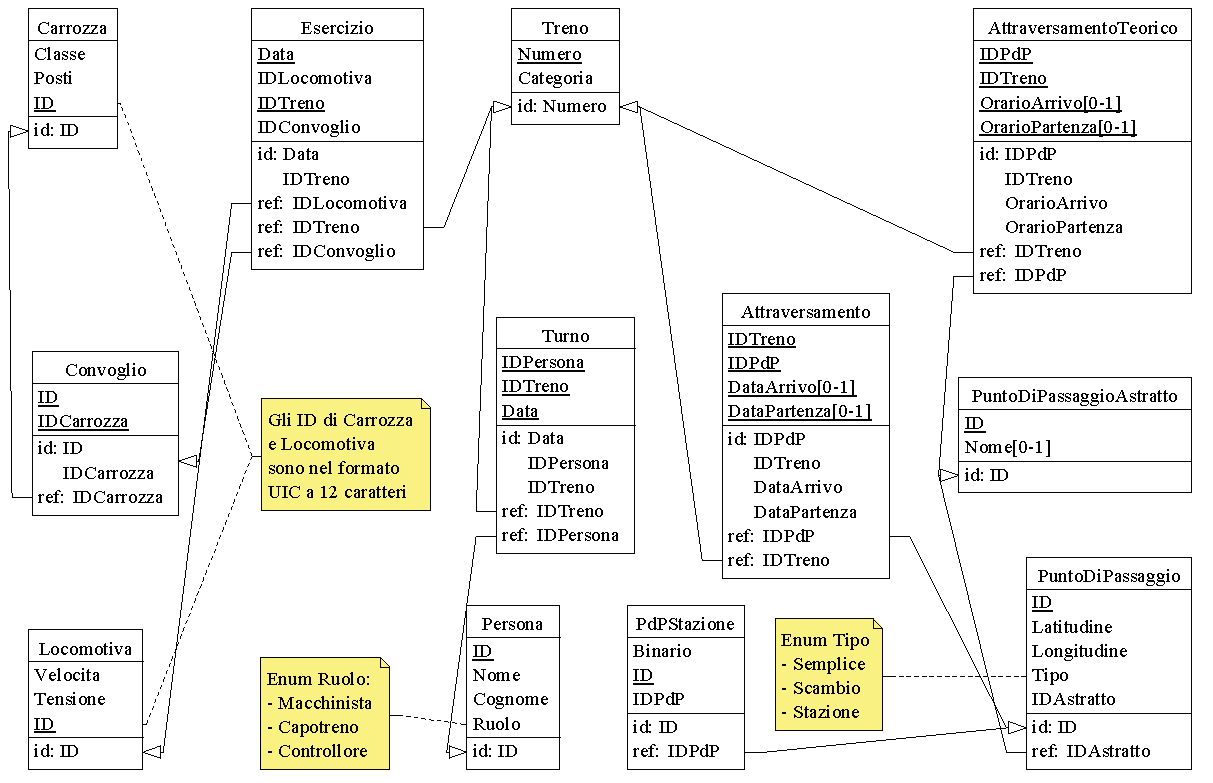
\includegraphics[width=\linewidth]{res/schema/logico}
		\end{center}
		\caption{Schema relazionale finale}
	\end{figure}
	\section{Traduzione delle operazioni in query SQL}
	

	\chapter{Progettazione dell'applicazione}
	\section{Descrizione dell'architettura dell'applicazione realizzata}
	\par Si sviluppa un interfaccia web per la gestione del sistema, sviluppata utilizzando il framework Bootstrap e l'approccio \textit{mobile-first}.
	\par Il linguaggio usato per il webserver che gestisce le richieste dell'interfaccia è il Rust.
	\\Il webserver si interfaccia al database tramite la crate postgres.
	\\Il DBMS usato e' PostgreSQL.
	\par Per ogni tabella si possono inserire righe tramite un form.
	\\Ogni tabella o view si puo visualizzare, anche ricercando campi.
	\par Dalla home page si possono anche cercare informazioni su treni e stazioni, che portano a pagine specifiche.

	\subsection{Homepage}
	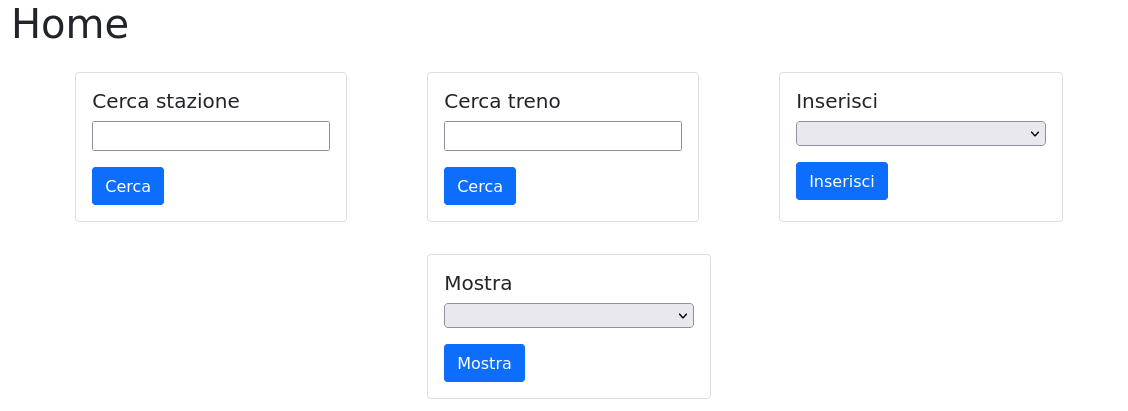
\includegraphics[width=\linewidth]{res/screenshots/home.png}
	\par Dalla homepage si puo accedere alle 2 funzioni principali di gestione del database: inserimento e ricerca,
	selezionando tramite un menu drop-down la tabella o view interessata.
	\par Si puo inoltre accedere a informazioni su treni e stazioni, con una ricerca con suggerimenti.
	\subsection{Inserimento}
	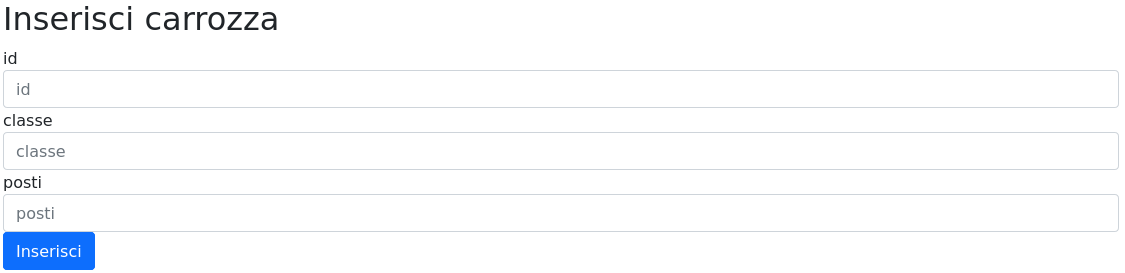
\includegraphics[width=\linewidth]{res/screenshots/inserisci.png}
	\par Nella pagina di inserimento, per ogni tabella, si puo compilare un form per inserire una riga alla tabella.
	\par Per foreign key presenti nella tabella, vengono suggeriti i valori da inserire.
	\subsection{Ricerca}
	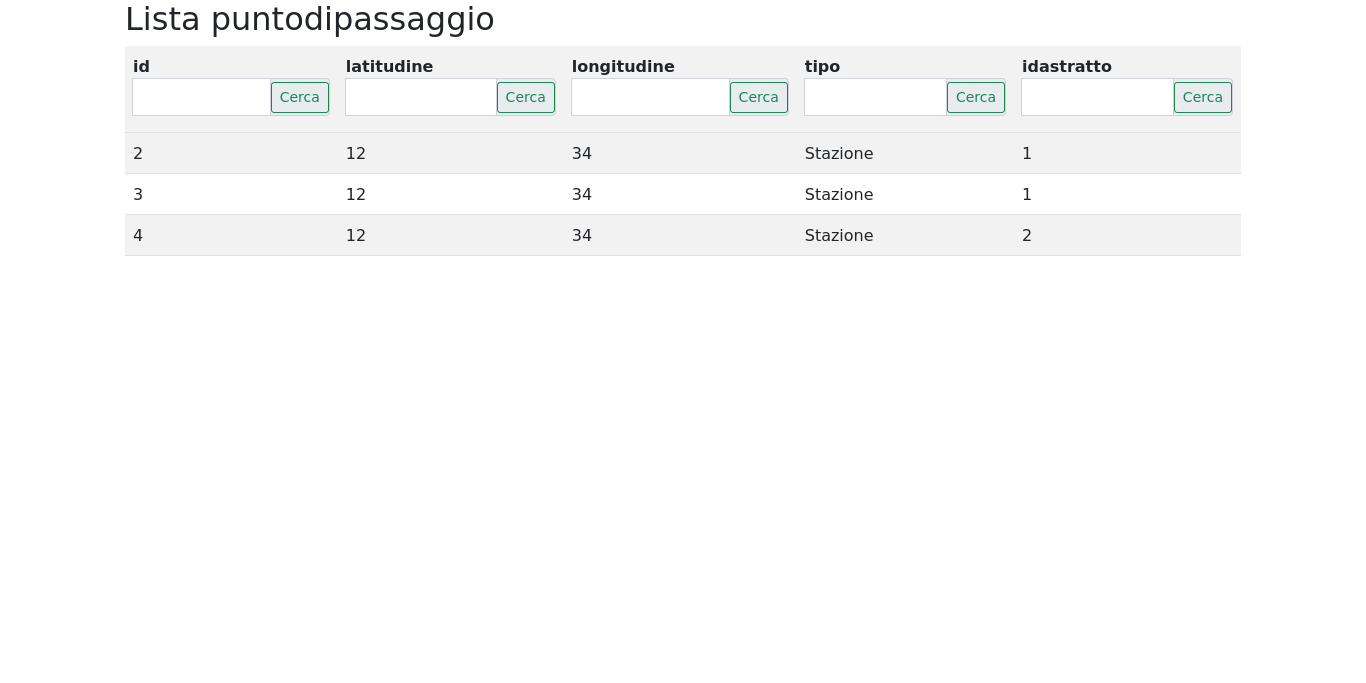
\includegraphics[width=\linewidth]{res/screenshots/lista.png}
	\par Nella pagina di ricerca viene visualizzata la tabella interessata.
	\par \`E possibile eseguire una ricerca per una qualsiasi colonna della tabella.
	\subsection{Ricerca stazione}
	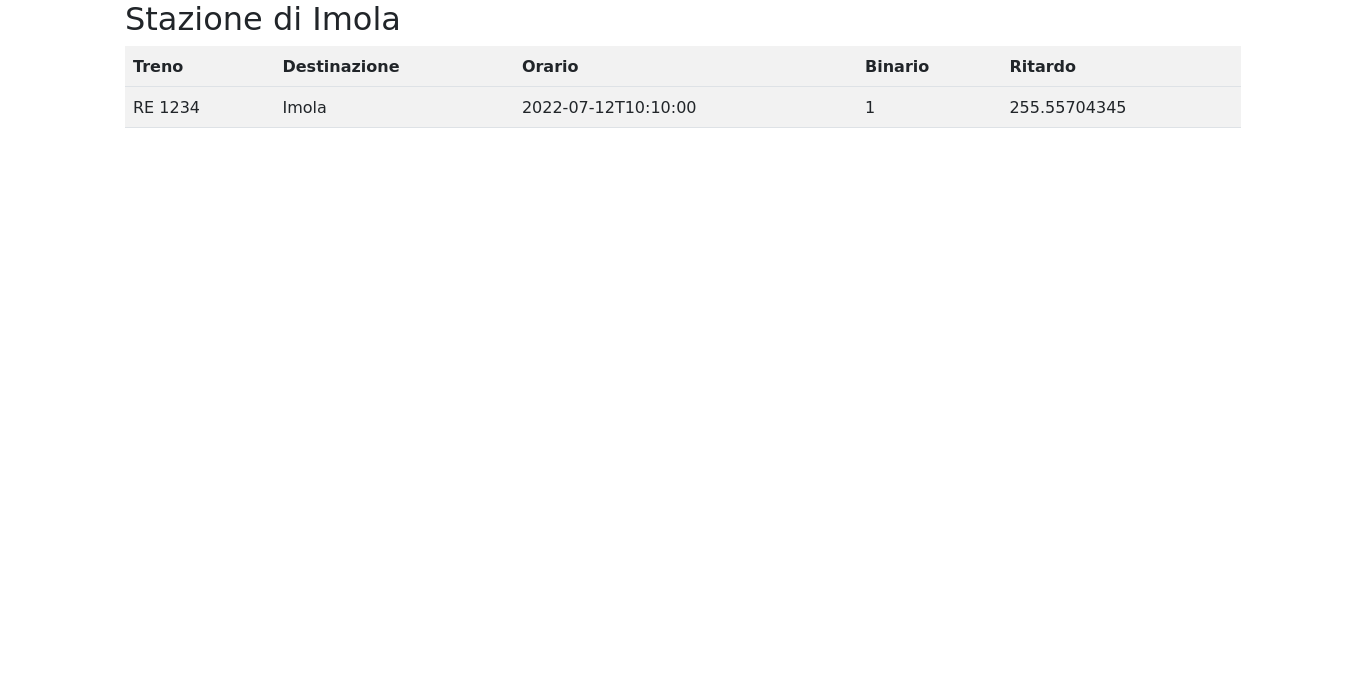
\includegraphics[width=\linewidth]{res/screenshots/stazione.png}
	\par Nella pagina relativa alla ricerca della stazione si puo vedere la lista dei treni che passano dalla stazione e alcune informazioni relative ad essi.
	\par Se si clicca sul numero del treno, si va alla pagina dello stato del treno nel giorno corrente.
	\subsection{Ricerca treno}
	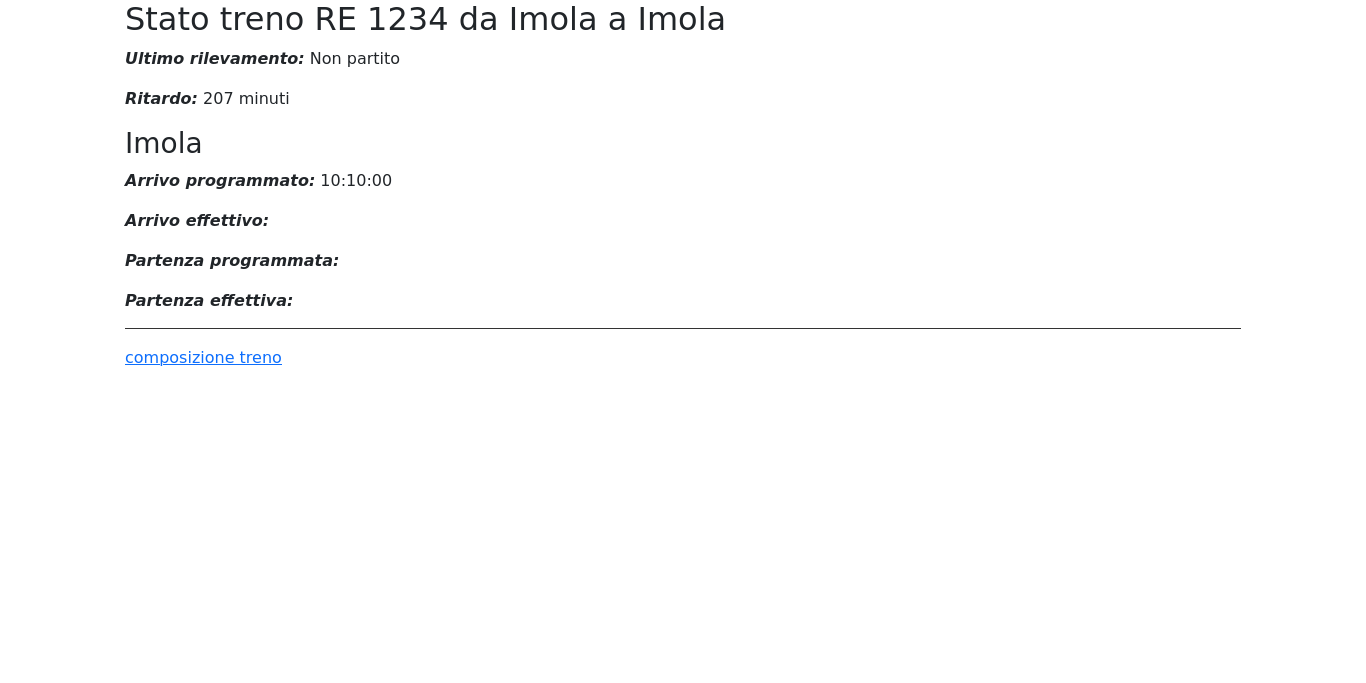
\includegraphics[width=\linewidth]{res/screenshots/stato_treno.png}
	\par Nella pagina relativa alla ricerca del treno si possono vedere informazioni logistiche relative allo stato del treno.
	\par \`E anche presente un link che manda a una pagina per visualizzare la composizione del treno stesso.
	\appendix
	\chapter{Istruzioni per l'installazione}
	\section{Prerequisiti}
	\begin{itemize}
		\item Un DBMS PostgreSQL con già creato un database vuoto
		\item Un utente che abbia i permessi di creazione tabelle e viste, di interrogazione e di inserimento sul database
	\end{itemize}
	\section{Configurazione}
	\par \`E necessario creare un file denominato \texttt{.env} nella cartella in cui verrà eseguito il programma, contenente nel formato \texttt{<KEY>=<VALUE>} (una variabile per riga) le seguenti variabili:
	\begin{itemize}
		\item \texttt{DB\_HOST}: l'indirizzo IP o l'hostname su cui è raggiungibile il DBMS,
		\item \texttt{DB\_NAME}: il nome del DB in cui verranno create le tabelle,
		\item \texttt{DB\_USER}: l'utente per autenticarsi al DB,
		\item \texttt{DB\_PASSWORD}: la password dell'utente sopra specificato.
	\end{itemize}
	\section{Esecuzione del programma}
	\par Dopo aver scaricato l'eseguibile per la piattaforma desiderata, controllare che abbia i permessi di esecuzione (se richiesti) ed eseguirlo nella cartella in cui è stato posizionato il file \texttt{.env} e la cartella \texttt{templates}.
	\par Il programma provvederà all'inizializzazione del DB e si metterà in ascolto sulla porta TCP 8000.
    %\printbibliography[heading=bibintoc]
    \listoffigures
\end{document}
